% Created by tikzDevice version 0.12.6 on 2025-01-17 13:26:23
% !TEX encoding = UTF-8 Unicode
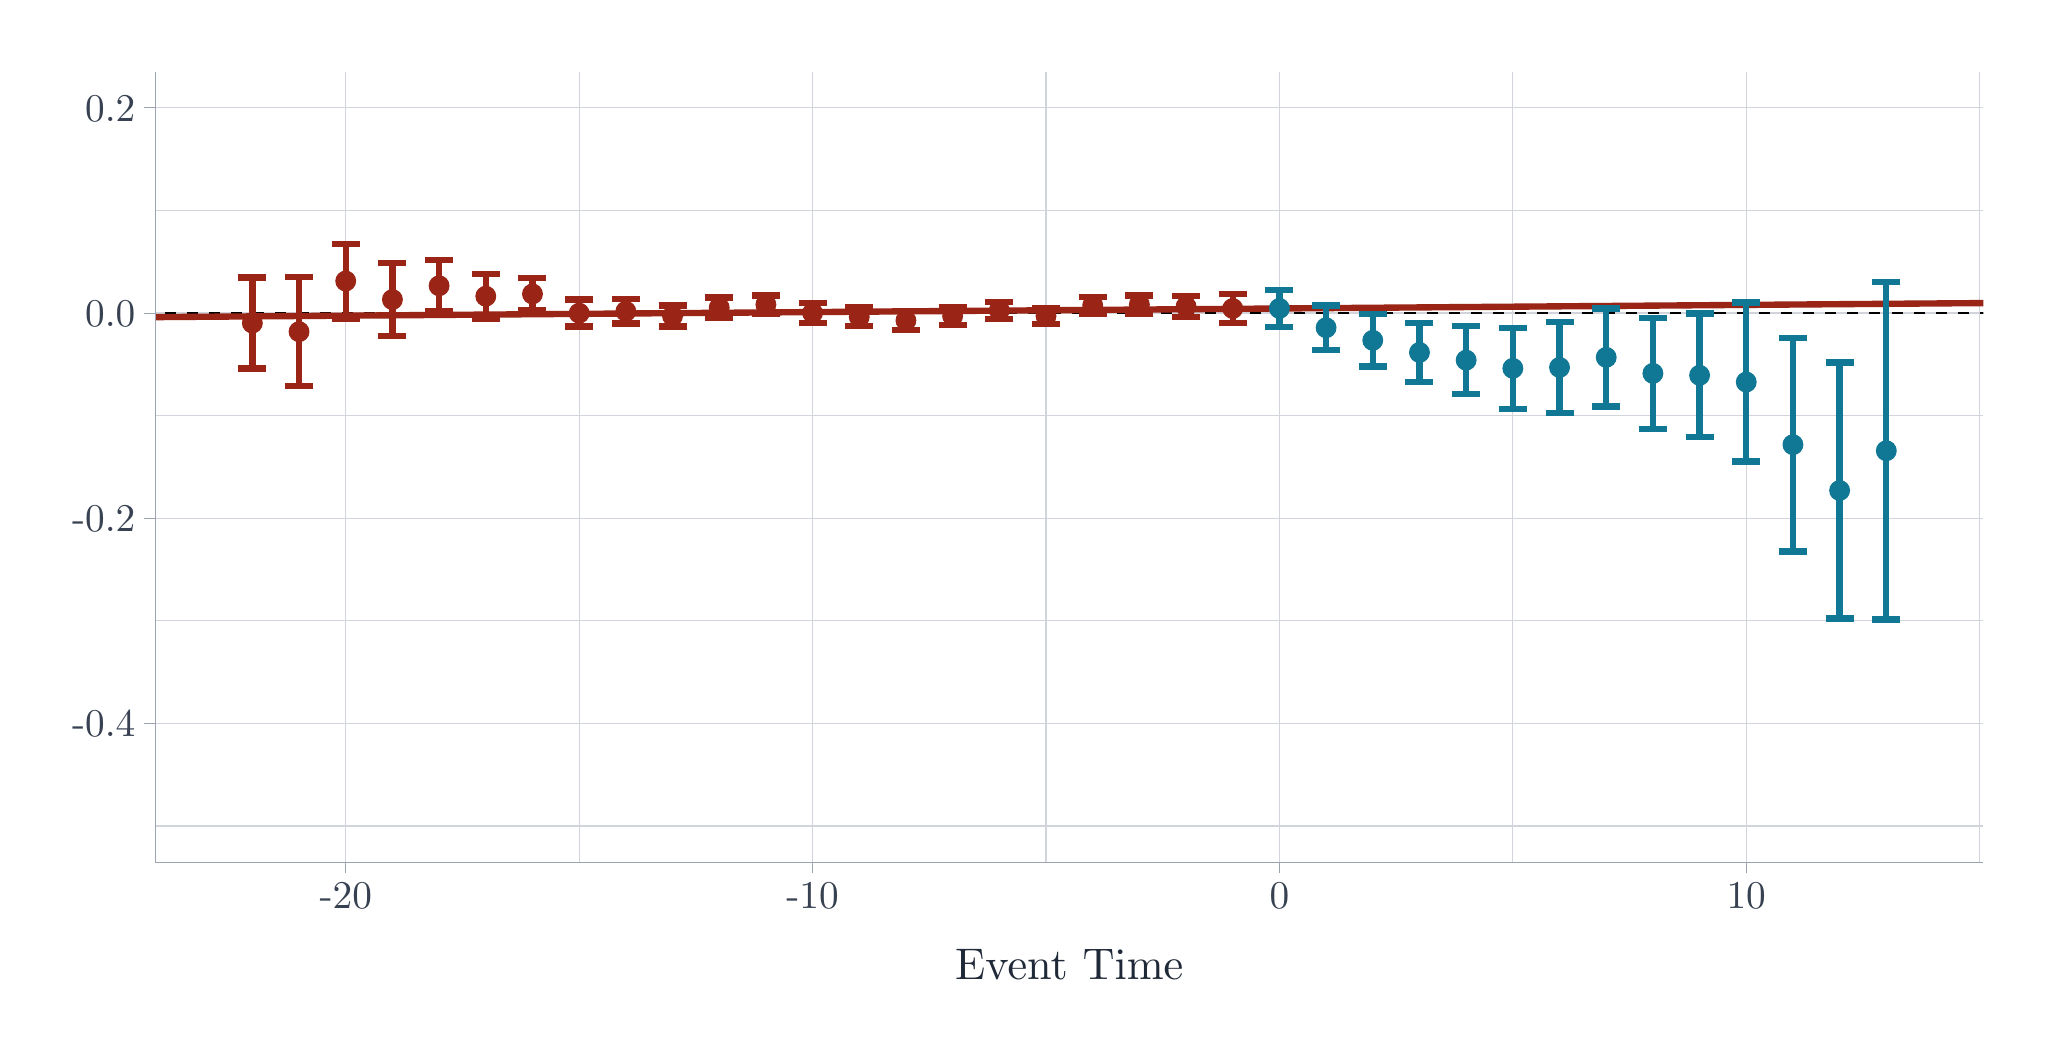
\begin{tikzpicture}[x=1pt,y=1pt]
\definecolor{fillColor}{RGB}{255,255,255}
\path[use as bounding box,fill=fillColor] (0,0) rectangle (722.70,361.35);
\begin{scope}
\path[clip] (  0.00,  0.00) rectangle (722.70,361.35);
\definecolor{drawColor}{RGB}{255,255,255}

\path[draw=drawColor,line width= 0.8pt,line join=round,line cap=round,fill=fillColor] (  0.00,  0.00) rectangle (722.70,361.35);
\end{scope}
\begin{scope}
\path[clip] ( 46.10, 59.89) rectangle (706.70,345.35);
\definecolor{drawColor}{RGB}{255,255,255}
\definecolor{fillColor}{RGB}{255,255,255}

\path[draw=drawColor,line width= 0.8pt,line join=round,line cap=round,fill=fillColor] ( 46.10, 59.89) rectangle (706.70,345.35);
\definecolor{drawColor}{RGB}{209,213,219}

\path[draw=drawColor,line width= 0.4pt,line join=round] ( 46.10, 72.86) --
	(706.70, 72.86);

\path[draw=drawColor,line width= 0.4pt,line join=round] ( 46.10,147.01) --
	(706.70,147.01);

\path[draw=drawColor,line width= 0.4pt,line join=round] ( 46.10,221.16) --
	(706.70,221.16);

\path[draw=drawColor,line width= 0.4pt,line join=round] ( 46.10,295.30) --
	(706.70,295.30);

\path[draw=drawColor,line width= 0.4pt,line join=round] (199.28, 59.89) --
	(199.28,345.35);

\path[draw=drawColor,line width= 0.4pt,line join=round] (367.97, 59.89) --
	(367.97,345.35);

\path[draw=drawColor,line width= 0.4pt,line join=round] (536.66, 59.89) --
	(536.66,345.35);

\path[draw=drawColor,line width= 0.4pt,line join=round] (705.35, 59.89) --
	(705.35,345.35);

\path[draw=drawColor,line width= 0.4pt,line join=round] ( 46.10,109.94) --
	(706.70,109.94);

\path[draw=drawColor,line width= 0.4pt,line join=round] ( 46.10,184.08) --
	(706.70,184.08);

\path[draw=drawColor,line width= 0.4pt,line join=round] ( 46.10,258.23) --
	(706.70,258.23);

\path[draw=drawColor,line width= 0.4pt,line join=round] ( 46.10,332.37) --
	(706.70,332.37);

\path[draw=drawColor,line width= 0.4pt,line join=round] (114.93, 59.89) --
	(114.93,345.35);

\path[draw=drawColor,line width= 0.4pt,line join=round] (283.62, 59.89) --
	(283.62,345.35);

\path[draw=drawColor,line width= 0.4pt,line join=round] (452.31, 59.89) --
	(452.31,345.35);

\path[draw=drawColor,line width= 0.4pt,line join=round] (621.00, 59.89) --
	(621.00,345.35);
\definecolor{drawColor}{RGB}{0,0,0}

\path[draw=drawColor,line width= 0.9pt,dash pattern=on 4pt off 4pt ,line join=round] (-614.49,258.23) -- (1367.30,258.23);
\definecolor{drawColor}{RGB}{154,36,21}

\path[draw=drawColor,line width= 2.3pt,line join=round] (-614.49,251.67) -- (1367.30,266.91);
\definecolor{fillColor}{RGB}{154,36,21}

\path[draw=drawColor,line width= 0.4pt,line join=round,line cap=round,fill=fillColor] ( 81.19,254.61) circle (  3.57);

\path[draw=drawColor,line width= 0.4pt,line join=round,line cap=round,fill=fillColor] ( 98.06,251.49) circle (  3.57);

\path[draw=drawColor,line width= 0.4pt,line join=round,line cap=round,fill=fillColor] (114.93,269.80) circle (  3.57);

\path[draw=drawColor,line width= 0.4pt,line join=round,line cap=round,fill=fillColor] (131.80,263.10) circle (  3.57);

\path[draw=drawColor,line width= 0.4pt,line join=round,line cap=round,fill=fillColor] (148.67,268.08) circle (  3.57);

\path[draw=drawColor,line width= 0.4pt,line join=round,line cap=round,fill=fillColor] (165.54,264.31) circle (  3.57);

\path[draw=drawColor,line width= 0.4pt,line join=round,line cap=round,fill=fillColor] (182.41,265.12) circle (  3.57);

\path[draw=drawColor,line width= 0.4pt,line join=round,line cap=round,fill=fillColor] (199.28,258.18) circle (  3.57);

\path[draw=drawColor,line width= 0.4pt,line join=round,line cap=round,fill=fillColor] (216.15,258.85) circle (  3.57);

\path[draw=drawColor,line width= 0.4pt,line join=round,line cap=round,fill=fillColor] (233.01,257.15) circle (  3.57);

\path[draw=drawColor,line width= 0.4pt,line join=round,line cap=round,fill=fillColor] (249.88,260.18) circle (  3.57);

\path[draw=drawColor,line width= 0.4pt,line join=round,line cap=round,fill=fillColor] (266.75,261.28) circle (  3.57);

\path[draw=drawColor,line width= 0.4pt,line join=round,line cap=round,fill=fillColor] (283.62,258.27) circle (  3.57);

\path[draw=drawColor,line width= 0.4pt,line join=round,line cap=round,fill=fillColor] (300.49,256.83) circle (  3.57);

\path[draw=drawColor,line width= 0.4pt,line join=round,line cap=round,fill=fillColor] (317.36,255.52) circle (  3.57);

\path[draw=drawColor,line width= 0.4pt,line join=round,line cap=round,fill=fillColor] (334.23,257.13) circle (  3.57);

\path[draw=drawColor,line width= 0.4pt,line join=round,line cap=round,fill=fillColor] (351.10,259.20) circle (  3.57);

\path[draw=drawColor,line width= 0.4pt,line join=round,line cap=round,fill=fillColor] (367.97,257.16) circle (  3.57);

\path[draw=drawColor,line width= 0.4pt,line join=round,line cap=round,fill=fillColor] (384.84,261.00) circle (  3.57);

\path[draw=drawColor,line width= 0.4pt,line join=round,line cap=round,fill=fillColor] (401.71,261.33) circle (  3.57);

\path[draw=drawColor,line width= 0.4pt,line join=round,line cap=round,fill=fillColor] (418.58,260.60) circle (  3.57);

\path[draw=drawColor,line width= 0.4pt,line join=round,line cap=round,fill=fillColor] (435.44,259.87) circle (  3.57);
\definecolor{drawColor}{RGB}{16,120,149}
\definecolor{fillColor}{RGB}{16,120,149}

\path[draw=drawColor,line width= 0.4pt,line join=round,line cap=round,fill=fillColor] (452.31,259.90) circle (  3.57);

\path[draw=drawColor,line width= 0.4pt,line join=round,line cap=round,fill=fillColor] (469.18,252.92) circle (  3.57);

\path[draw=drawColor,line width= 0.4pt,line join=round,line cap=round,fill=fillColor] (486.05,248.37) circle (  3.57);

\path[draw=drawColor,line width= 0.4pt,line join=round,line cap=round,fill=fillColor] (502.92,243.99) circle (  3.57);

\path[draw=drawColor,line width= 0.4pt,line join=round,line cap=round,fill=fillColor] (519.79,241.21) circle (  3.57);

\path[draw=drawColor,line width= 0.4pt,line join=round,line cap=round,fill=fillColor] (536.66,238.25) circle (  3.57);

\path[draw=drawColor,line width= 0.4pt,line join=round,line cap=round,fill=fillColor] (553.53,238.57) circle (  3.57);

\path[draw=drawColor,line width= 0.4pt,line join=round,line cap=round,fill=fillColor] (570.40,242.22) circle (  3.57);

\path[draw=drawColor,line width= 0.4pt,line join=round,line cap=round,fill=fillColor] (587.27,236.44) circle (  3.57);

\path[draw=drawColor,line width= 0.4pt,line join=round,line cap=round,fill=fillColor] (604.14,235.73) circle (  3.57);

\path[draw=drawColor,line width= 0.4pt,line join=round,line cap=round,fill=fillColor] (621.00,233.30) circle (  3.57);

\path[draw=drawColor,line width= 0.4pt,line join=round,line cap=round,fill=fillColor] (637.87,210.67) circle (  3.57);

\path[draw=drawColor,line width= 0.4pt,line join=round,line cap=round,fill=fillColor] (654.74,194.11) circle (  3.57);

\path[draw=drawColor,line width= 0.4pt,line join=round,line cap=round,fill=fillColor] (671.61,208.47) circle (  3.57);
\definecolor{drawColor}{RGB}{154,36,21}

\path[draw=drawColor,line width= 2.3pt,line join=round] ( 76.13,271.08) --
	( 86.25,271.08);

\path[draw=drawColor,line width= 2.3pt,line join=round] ( 81.19,271.08) --
	( 81.19,238.15);

\path[draw=drawColor,line width= 2.3pt,line join=round] ( 76.13,238.15) --
	( 86.25,238.15);

\path[draw=drawColor,line width= 2.3pt,line join=round] ( 93.00,271.16) --
	(103.12,271.16);

\path[draw=drawColor,line width= 2.3pt,line join=round] ( 98.06,271.16) --
	( 98.06,231.83);

\path[draw=drawColor,line width= 2.3pt,line join=round] ( 93.00,231.83) --
	(103.12,231.83);

\path[draw=drawColor,line width= 2.3pt,line join=round] (109.87,283.29) --
	(119.99,283.29);

\path[draw=drawColor,line width= 2.3pt,line join=round] (114.93,283.29) --
	(114.93,256.31);

\path[draw=drawColor,line width= 2.3pt,line join=round] (109.87,256.31) --
	(119.99,256.31);

\path[draw=drawColor,line width= 2.3pt,line join=round] (126.74,276.20) --
	(136.86,276.20);

\path[draw=drawColor,line width= 2.3pt,line join=round] (131.80,276.20) --
	(131.80,250.00);

\path[draw=drawColor,line width= 2.3pt,line join=round] (126.74,250.00) --
	(136.86,250.00);

\path[draw=drawColor,line width= 2.3pt,line join=round] (143.61,277.35) --
	(153.73,277.35);

\path[draw=drawColor,line width= 2.3pt,line join=round] (148.67,277.35) --
	(148.67,258.81);

\path[draw=drawColor,line width= 2.3pt,line join=round] (143.61,258.81) --
	(153.73,258.81);

\path[draw=drawColor,line width= 2.3pt,line join=round] (160.48,272.39) --
	(170.60,272.39);

\path[draw=drawColor,line width= 2.3pt,line join=round] (165.54,272.39) --
	(165.54,256.23);

\path[draw=drawColor,line width= 2.3pt,line join=round] (160.48,256.23) --
	(170.60,256.23);

\path[draw=drawColor,line width= 2.3pt,line join=round] (177.35,270.97) --
	(187.47,270.97);

\path[draw=drawColor,line width= 2.3pt,line join=round] (182.41,270.97) --
	(182.41,259.27);

\path[draw=drawColor,line width= 2.3pt,line join=round] (177.35,259.27) --
	(187.47,259.27);

\path[draw=drawColor,line width= 2.3pt,line join=round] (194.22,263.06) --
	(204.34,263.06);

\path[draw=drawColor,line width= 2.3pt,line join=round] (199.28,263.06) --
	(199.28,253.30);

\path[draw=drawColor,line width= 2.3pt,line join=round] (194.22,253.30) --
	(204.34,253.30);

\path[draw=drawColor,line width= 2.3pt,line join=round] (211.08,263.21) --
	(221.21,263.21);

\path[draw=drawColor,line width= 2.3pt,line join=round] (216.15,263.21) --
	(216.15,254.49);

\path[draw=drawColor,line width= 2.3pt,line join=round] (211.08,254.49) --
	(221.21,254.49);

\path[draw=drawColor,line width= 2.3pt,line join=round] (227.95,260.99) --
	(238.08,260.99);

\path[draw=drawColor,line width= 2.3pt,line join=round] (233.01,260.99) --
	(233.01,253.31);

\path[draw=drawColor,line width= 2.3pt,line join=round] (227.95,253.31) --
	(238.08,253.31);

\path[draw=drawColor,line width= 2.3pt,line join=round] (244.82,263.88) --
	(254.94,263.88);

\path[draw=drawColor,line width= 2.3pt,line join=round] (249.88,263.88) --
	(249.88,256.47);

\path[draw=drawColor,line width= 2.3pt,line join=round] (244.82,256.47) --
	(254.94,256.47);

\path[draw=drawColor,line width= 2.3pt,line join=round] (261.69,264.55) --
	(271.81,264.55);

\path[draw=drawColor,line width= 2.3pt,line join=round] (266.75,264.55) --
	(266.75,258.00);

\path[draw=drawColor,line width= 2.3pt,line join=round] (261.69,258.00) --
	(271.81,258.00);

\path[draw=drawColor,line width= 2.3pt,line join=round] (278.56,261.87) --
	(288.68,261.87);

\path[draw=drawColor,line width= 2.3pt,line join=round] (283.62,261.87) --
	(283.62,254.67);

\path[draw=drawColor,line width= 2.3pt,line join=round] (278.56,254.67) --
	(288.68,254.67);

\path[draw=drawColor,line width= 2.3pt,line join=round] (295.43,260.19) --
	(305.55,260.19);

\path[draw=drawColor,line width= 2.3pt,line join=round] (300.49,260.19) --
	(300.49,253.46);

\path[draw=drawColor,line width= 2.3pt,line join=round] (295.43,253.46) --
	(305.55,253.46);

\path[draw=drawColor,line width= 2.3pt,line join=round] (312.30,258.92) --
	(322.42,258.92);

\path[draw=drawColor,line width= 2.3pt,line join=round] (317.36,258.92) --
	(317.36,252.12);

\path[draw=drawColor,line width= 2.3pt,line join=round] (312.30,252.12) --
	(322.42,252.12);

\path[draw=drawColor,line width= 2.3pt,line join=round] (329.17,260.46) --
	(339.29,260.46);

\path[draw=drawColor,line width= 2.3pt,line join=round] (334.23,260.46) --
	(334.23,253.80);

\path[draw=drawColor,line width= 2.3pt,line join=round] (329.17,253.80) --
	(339.29,253.80);

\path[draw=drawColor,line width= 2.3pt,line join=round] (346.04,262.30) --
	(356.16,262.30);

\path[draw=drawColor,line width= 2.3pt,line join=round] (351.10,262.30) --
	(351.10,256.10);

\path[draw=drawColor,line width= 2.3pt,line join=round] (346.04,256.10) --
	(356.16,256.10);

\path[draw=drawColor,line width= 2.3pt,line join=round] (362.91,260.09) --
	(373.03,260.09);

\path[draw=drawColor,line width= 2.3pt,line join=round] (367.97,260.09) --
	(367.97,254.24);

\path[draw=drawColor,line width= 2.3pt,line join=round] (362.91,254.24) --
	(373.03,254.24);

\path[draw=drawColor,line width= 2.3pt,line join=round] (379.78,264.03) --
	(389.90,264.03);

\path[draw=drawColor,line width= 2.3pt,line join=round] (384.84,264.03) --
	(384.84,257.97);

\path[draw=drawColor,line width= 2.3pt,line join=round] (379.78,257.97) --
	(389.90,257.97);

\path[draw=drawColor,line width= 2.3pt,line join=round] (396.65,264.60) --
	(406.77,264.60);

\path[draw=drawColor,line width= 2.3pt,line join=round] (401.71,264.60) --
	(401.71,258.06);

\path[draw=drawColor,line width= 2.3pt,line join=round] (396.65,258.06) --
	(406.77,258.06);

\path[draw=drawColor,line width= 2.3pt,line join=round] (413.51,264.44) --
	(423.64,264.44);

\path[draw=drawColor,line width= 2.3pt,line join=round] (418.58,264.44) --
	(418.58,256.76);

\path[draw=drawColor,line width= 2.3pt,line join=round] (413.51,256.76) --
	(423.64,256.76);

\path[draw=drawColor,line width= 2.3pt,line join=round] (430.38,265.02) --
	(440.50,265.02);

\path[draw=drawColor,line width= 2.3pt,line join=round] (435.44,265.02) --
	(435.44,254.73);

\path[draw=drawColor,line width= 2.3pt,line join=round] (430.38,254.73) --
	(440.50,254.73);
\definecolor{drawColor}{RGB}{16,120,149}

\path[draw=drawColor,line width= 2.3pt,line join=round] (447.25,266.53) --
	(457.37,266.53);

\path[draw=drawColor,line width= 2.3pt,line join=round] (452.31,266.53) --
	(452.31,253.27);

\path[draw=drawColor,line width= 2.3pt,line join=round] (447.25,253.27) --
	(457.37,253.27);

\path[draw=drawColor,line width= 2.3pt,line join=round] (464.12,260.96) --
	(474.24,260.96);

\path[draw=drawColor,line width= 2.3pt,line join=round] (469.18,260.96) --
	(469.18,244.88);

\path[draw=drawColor,line width= 2.3pt,line join=round] (464.12,244.88) --
	(474.24,244.88);

\path[draw=drawColor,line width= 2.3pt,line join=round] (480.99,257.83) --
	(491.11,257.83);

\path[draw=drawColor,line width= 2.3pt,line join=round] (486.05,257.83) --
	(486.05,238.91);

\path[draw=drawColor,line width= 2.3pt,line join=round] (480.99,238.91) --
	(491.11,238.91);

\path[draw=drawColor,line width= 2.3pt,line join=round] (497.86,254.68) --
	(507.98,254.68);

\path[draw=drawColor,line width= 2.3pt,line join=round] (502.92,254.68) --
	(502.92,233.30);

\path[draw=drawColor,line width= 2.3pt,line join=round] (497.86,233.30) --
	(507.98,233.30);

\path[draw=drawColor,line width= 2.3pt,line join=round] (514.73,253.55) --
	(524.85,253.55);

\path[draw=drawColor,line width= 2.3pt,line join=round] (519.79,253.55) --
	(519.79,228.87);

\path[draw=drawColor,line width= 2.3pt,line join=round] (514.73,228.87) --
	(524.85,228.87);

\path[draw=drawColor,line width= 2.3pt,line join=round] (531.60,252.88) --
	(541.72,252.88);

\path[draw=drawColor,line width= 2.3pt,line join=round] (536.66,252.88) --
	(536.66,223.62);

\path[draw=drawColor,line width= 2.3pt,line join=round] (531.60,223.62) --
	(541.72,223.62);

\path[draw=drawColor,line width= 2.3pt,line join=round] (548.47,255.01) --
	(558.59,255.01);

\path[draw=drawColor,line width= 2.3pt,line join=round] (553.53,255.01) --
	(553.53,222.13);

\path[draw=drawColor,line width= 2.3pt,line join=round] (548.47,222.13) --
	(558.59,222.13);

\path[draw=drawColor,line width= 2.3pt,line join=round] (565.34,259.93) --
	(575.46,259.93);

\path[draw=drawColor,line width= 2.3pt,line join=round] (570.40,259.93) --
	(570.40,224.51);

\path[draw=drawColor,line width= 2.3pt,line join=round] (565.34,224.51) --
	(575.46,224.51);

\path[draw=drawColor,line width= 2.3pt,line join=round] (582.21,256.52) --
	(592.33,256.52);

\path[draw=drawColor,line width= 2.3pt,line join=round] (587.27,256.52) --
	(587.27,216.37);

\path[draw=drawColor,line width= 2.3pt,line join=round] (582.21,216.37) --
	(592.33,216.37);

\path[draw=drawColor,line width= 2.3pt,line join=round] (599.07,258.06) --
	(609.20,258.06);

\path[draw=drawColor,line width= 2.3pt,line join=round] (604.14,258.06) --
	(604.14,213.40);

\path[draw=drawColor,line width= 2.3pt,line join=round] (599.07,213.40) --
	(609.20,213.40);

\path[draw=drawColor,line width= 2.3pt,line join=round] (615.94,262.00) --
	(626.07,262.00);

\path[draw=drawColor,line width= 2.3pt,line join=round] (621.00,262.00) --
	(621.00,204.61);

\path[draw=drawColor,line width= 2.3pt,line join=round] (615.94,204.61) --
	(626.07,204.61);

\path[draw=drawColor,line width= 2.3pt,line join=round] (632.81,249.25) --
	(642.93,249.25);

\path[draw=drawColor,line width= 2.3pt,line join=round] (637.87,249.25) --
	(637.87,172.09);

\path[draw=drawColor,line width= 2.3pt,line join=round] (632.81,172.09) --
	(642.93,172.09);

\path[draw=drawColor,line width= 2.3pt,line join=round] (649.68,240.41) --
	(659.80,240.41);

\path[draw=drawColor,line width= 2.3pt,line join=round] (654.74,240.41) --
	(654.74,147.81);

\path[draw=drawColor,line width= 2.3pt,line join=round] (649.68,147.81) --
	(659.80,147.81);

\path[draw=drawColor,line width= 2.3pt,line join=round] (666.55,269.41) --
	(676.67,269.41);

\path[draw=drawColor,line width= 2.3pt,line join=round] (671.61,269.41) --
	(671.61,147.52);

\path[draw=drawColor,line width= 2.3pt,line join=round] (666.55,147.52) --
	(676.67,147.52);
\end{scope}
\begin{scope}
\path[clip] (  0.00,  0.00) rectangle (722.70,361.35);
\definecolor{drawColor}{RGB}{156,163,175}

\path[draw=drawColor,line width= 0.3pt,line join=round] ( 46.10, 59.89) --
	( 46.10,345.35);
\end{scope}
\begin{scope}
\path[clip] (  0.00,  0.00) rectangle (722.70,361.35);
\definecolor{drawColor}{RGB}{55,65,81}

\node[text=drawColor,anchor=base east,inner sep=0pt, outer sep=0pt, scale=  1.42] at ( 38.90,105.04) {-0.4};

\node[text=drawColor,anchor=base east,inner sep=0pt, outer sep=0pt, scale=  1.42] at ( 38.90,179.19) {-0.2};

\node[text=drawColor,anchor=base east,inner sep=0pt, outer sep=0pt, scale=  1.42] at ( 38.90,253.33) {0.0};

\node[text=drawColor,anchor=base east,inner sep=0pt, outer sep=0pt, scale=  1.42] at ( 38.90,327.48) {0.2};
\end{scope}
\begin{scope}
\path[clip] (  0.00,  0.00) rectangle (722.70,361.35);
\definecolor{drawColor}{RGB}{156,163,175}

\path[draw=drawColor,line width= 0.3pt,line join=round] ( 42.10,109.94) --
	( 46.10,109.94);

\path[draw=drawColor,line width= 0.3pt,line join=round] ( 42.10,184.08) --
	( 46.10,184.08);

\path[draw=drawColor,line width= 0.3pt,line join=round] ( 42.10,258.23) --
	( 46.10,258.23);

\path[draw=drawColor,line width= 0.3pt,line join=round] ( 42.10,332.37) --
	( 46.10,332.37);
\end{scope}
\begin{scope}
\path[clip] (  0.00,  0.00) rectangle (722.70,361.35);
\definecolor{drawColor}{RGB}{156,163,175}

\path[draw=drawColor,line width= 0.3pt,line join=round] ( 46.10, 59.89) --
	(706.70, 59.89);
\end{scope}
\begin{scope}
\path[clip] (  0.00,  0.00) rectangle (722.70,361.35);
\definecolor{drawColor}{RGB}{156,163,175}

\path[draw=drawColor,line width= 0.3pt,line join=round] (114.93, 55.89) --
	(114.93, 59.89);

\path[draw=drawColor,line width= 0.3pt,line join=round] (283.62, 55.89) --
	(283.62, 59.89);

\path[draw=drawColor,line width= 0.3pt,line join=round] (452.31, 55.89) --
	(452.31, 59.89);

\path[draw=drawColor,line width= 0.3pt,line join=round] (621.00, 55.89) --
	(621.00, 59.89);
\end{scope}
\begin{scope}
\path[clip] (  0.00,  0.00) rectangle (722.70,361.35);
\definecolor{drawColor}{RGB}{55,65,81}

\node[text=drawColor,anchor=base,inner sep=0pt, outer sep=0pt, scale=  1.42] at (114.93, 42.89) {-20};

\node[text=drawColor,anchor=base,inner sep=0pt, outer sep=0pt, scale=  1.42] at (283.62, 42.89) {-10};

\node[text=drawColor,anchor=base,inner sep=0pt, outer sep=0pt, scale=  1.42] at (452.31, 42.89) {0};

\node[text=drawColor,anchor=base,inner sep=0pt, outer sep=0pt, scale=  1.42] at (621.00, 42.89) {10};
\end{scope}
\begin{scope}
\path[clip] (  0.00,  0.00) rectangle (722.70,361.35);
\definecolor{drawColor}{RGB}{31,41,55}

\node[text=drawColor,anchor=base,inner sep=0pt, outer sep=0pt, scale=  1.60] at (376.40, 17.56) {Event Time};
\end{scope}
\end{tikzpicture}
